\documentclass[aspectratio=169]{beamer}
\usepackage{graphicx} % Required for inserting images

% \usepackage{armtex}
\usepackage{amsmath}
\usepackage{amsthm}
\usepackage{tikz}
% \usepackage{xcolor}

% \usepackage[usenames,dvipsnames]{xcolor}
\usepackage{algorithm}
\usepackage{algpseudocode}
\usepackage{array}
\usepackage{longtable}
\usepackage{booktabs}
\usepackage{url}
\newcommand{\doi}[1]{\texttt{doi:#1}}
\makeatletter
\def\thmhead@plain#1#2#3{%
  \thmname{#1}\thmnumber{\@ifnotempty{#1}{ }\@upn{#2}}%
  \thmnote{ {\the\thm@notefont#3}}}
\let\thmhead\thmhead@plain
\makeatother

\newcommand{\red}[1]{\textcolor{red}{#1}}
\newcommand{\blue}[1]{\textcolor{blue}{#1}}
\newcommand{\yellow}[1]{\textcolor{yellow}{#1}}
\newcommand{\violet}[1]{\textcolor{violet}{#1}}
\newcommand{\orange}[1]{\textcolor{orange}{#1}}
\newcommand{\green}[1]{\textcolor{green}{#1}}

% ----------------------------\

\usepackage{amsmath}
% \beamertemplatenavigationsymbolsempty

\usetheme{Malmoe}

%gets rid of bottom navigation bars
\setbeamertemplate{footline}[frame number]{}

% %gets rid of bottom navigation symbols
\setbeamertemplate{navigation symbols}{}

%gets rid of footer
%will override 'frame number' instruction above
%comment out to revert to previous/default definitions
\setbeamertemplate{footline}{}

\title{DSGD++: Reducing Uncertainty and Training Time in the DSGD Classifier through a Mass Assignment Function Initialization Technique}
\author{Tarkhanyan, A. and Harutyunyan, A.}
\date{\today}

\begin{document}

\begin{frame}
  \titlepage
\end{frame}

\begin{frame}
{\small\tableofcontents}
\end{frame}

\begin{frame}
    \begin{center}
        \Huge Dempster-Shafer theory
    \end{center}
\end{frame}

\section{Dempster-Shafer theory (DST)}
\begin{frame}{Dempster-Shafer theory (DST)}
    \begin{block}{General description of DST}
        DST (also known as "theory of belief functions") provides a
mathematical approach for combining evidence from different sources to calculate
the probability of an event, utilizing Dempster's rule of combination. 
        
    \end{block}
\end{frame}


\subsection{Mass Assignment functions}
\begin{frame}{Mass Assignment Function (MAF)}
  \begin{itemize}
    \item \textbf{Mathematical formulation:}
      \begin{itemize}
        \item Let \( X \) be the set of events, known as the frame of discernment. \pause
        \item The mass assignment function \( m \) is a function defined on the set of subsets of \( X \), \( 2^X \), such that:
          \[
          m : 2^X \rightarrow [0, 1]
          \]
        \pause
        \item The following conditions hold:
          \begin{enumerate}
            \item \( m(\emptyset) = 0 \) (The empty set has no mass)
            \item \( \sum\limits_{A \subseteq X} m(A) = 1 \) (The sum of masses is always 1)
          \end{enumerate}
      \end{itemize}
  \end{itemize}
\end{frame}

\begin{frame}{Examples of MAF}
\begin{itemize}
    \item Imagine we are flipping a fair coin. In a classic probability model, this can be expressed as $P(\{heads\}) = P(\{tails\}) = 0.5$. In the DST model, it would be $m(\emptyset) = 0, m(\{heads\}) = m(\{tails\}) = 0.5, m(\{heads, tails\}) = 0$.
    \pause
    \item If the coin were unfair, with the classic approach we could not assert anything, whereas with DST we can say that $m(\emptyset) = 0, m(\{heads\}) = m(\{tails\}) = 0, m(\{heads, tails\}) = 1$.
    \pause
    \item An example where DST can shine is the following. Imagine a person has seen a car passing by and makes the following statement:
    \begin{enumerate}
        \item The car was either black or brown, in any case, it seemed to be black, but I might be mistaken.
        In this case, the MAF could look like this: $m(\{\emptyset\}) = 0.1, m(\{ black\}) = 0.4, m(\{ brown\}) = 0.3, m(\{ black, brown\}) = 0.2$
    \end{enumerate}
\end{itemize}
\end{frame}

\subsection{Belief and Plausibility}
\begin{frame}{Belief and Plausibility}
    \begin{block}{}
         For all \( A \subseteq X \):
          \[
          Bel(A) = \sum_{B \subseteq A} m(B)
          \]
        \[
          Pl(A) = \sum_{B \cap A \neq \emptyset} m(B)
          \]
            \[
            Bel(A) \le P(A) \le Pl(A)
            \]

    In the previous example for the black car, we would have:
    $m(\{\emptyset\}) = 0.1, m(\{ black\}) = 0.4, m(\{ brown\}) = 0.3, m(\{ black, brown\}) = 0.2$ \\
    Let $A$ = black, $B$ = brown
          \[
        Bel(A) = m(A) = 0.4 \]
        \[
        Pl(A) = m(A) + m(\{A, B\}) = 0.4 + 0.2 = 0.6
          \]
    \end{block}
\end{frame}

\subsection{Dempster's Rule of Combination}
\begin{frame}{Dempster's Rule of Combination}
\begin{itemize}
  \item Dempster's rule is used to combine two mass assignment functions \(m_1\) and \(m_2\) into a new one \(m_f\).
  \item \textbf{Formula:}
    \begin{equation*}
      m_f(A) = m_1(A) \oplus m_2(A) = \frac{1}{1 - K} \sum_{B \cap C = A} m_1(B) m_2(C)
    \end{equation*}
    \pause
  \item \textbf{Measure of conflict \(K\):}
    \begin{equation*}
      K = \sum_{B \cap C = \emptyset} m_1(B) m_2(C)
    \end{equation*}
    \pause
  \item If $K=1$, it leads to a division by zero problem, indicating complete conflict between the evidence.
  \end{itemize}
\end{frame}

\section{Old Approach}

\begin{frame}
    \begin{center}
        \Huge Old approach
    \end{center}
\end{frame}

\begin{frame}{Old approach}
    In order to get the prediction
\begin{enumerate}
    \item For the given dataset $RS$ rule set is generated.
    \item Each rule's corresponding $MAF$ gets initiated in the following way: Uncertainty (whole set) gets 0.8 weight, and the remaining 0.2 weight is randomly split between $singleton$ elements.
    \item For given input $x$:
\end{enumerate}
\end{frame}

\begin{frame}
\begin{figure}
    \centering
    \includegraphics[width=0.45\linewidth]{../../fig/image.png}
    \label{fig:image}
\end{figure}
\end{frame}

\begin{frame}{Old approach}
\begin{align*}
\mathcal{M}_x &= \left\{ m \mid (m, s) \in RS \land x \right\} \\
m_f &= \bigoplus_{m \in \mathcal{M}_x} m \\
\hat{y} &= \underset{{\rm class}}{\mathrm{argmax}} \, {\rm Bel}(m_f)
\end{align*}
\end{frame}

\begin{frame}{Loss function}
    \begin{block}{Mean squared error}
        \begin{equation}
MSE = \frac{1}{n} \sum_{i=1}^{n} \left\| y_i - \hat{y}_i \right\|^2
        \end{equation}
    \end{block}
    \begin{block}{Cross-Entropy}
        \begin{equation}
        CE = - \frac{1}{n} \sum_{i=1}^{n} \sum_{j=1}^{k} y_{ij} \cdot \log(\hat{y}_{ij})
        \end{equation}
    \end{block}
\end{frame}

\begin{frame}
\begin{figure}
    \centering
    \includegraphics[width=0.55\linewidth]{../../fig/dst_ill_eng.png}
\end{figure}
\end{frame}

\section{Our approach}
\begin{frame}
    \begin{center}
        \Huge Our approach
    \end{center}
\end{frame}

\subsection{KMeans}
\begin{frame}
\begin{figure}
    \centering
    \includegraphics[width=0.68\linewidth]{../../fig/alg_kmeans_opacity.png}
    \caption{KMeans Algorithm}
    \label{fig:alg_kmeans}
\end{figure}
\end{frame}

\begin{frame}
\begin{figure}
    \centering
    \includegraphics[width=0.78\linewidth]{../../fig/kmeans_opactiy.png}
    \label{fig:kmeans_opacity}
\end{figure}
\end{frame}

\subsection{DBSCAN}
\begin{frame}
\begin{figure}
    \centering
    \includegraphics[width=0.75\linewidth]{../../fig/alg_dbscan_opacity.png}
    \label{fig:alg_dbscan}
\end{figure}
\end{frame}

\begin{frame}
\begin{figure}
    \centering
    \includegraphics[width=0.75\linewidth]{../../fig/denisty_opactiy.png}
    \label{fig:density_opacity}
\end{figure}
\end{frame}

\subsection{Rule confidence estimation}
\begin{frame}{Rule confidence estimation}
\begin{enumerate}
    \item Filter the dataset to retain only the rows that comply with the rule. \pause
    \item If the rule does not apply to any rows, set its confidence to 0 (this corresponds to the full uncertainty). Otherwise: \pause
    \item Calculate the rule's confidence as the mean representativeness of the rows it covers. \pause
    \item If the rows are not homogeneous with respect to their labels, reduce the confidence based on the proportion of the most frequent label among these rows.
\end{enumerate} 
\end{frame}

\subsection{MAF Initialization}
\begin{frame}{MAF Initialization}
\[
m(l_i) = 
\begin{cases} 
c & \text{if } l_i = l_{\text{mode}}, \\
\frac{1-c}{n-1} & \text{otherwise},
\end{cases}
\]
\end{frame}

\section{Results}

\begin{frame}
    \begin{center}
        \Huge Results
    \end{center}
\end{frame}

\subsection{Data}
\begin{frame}{Data}
{\rm
\begin{longtable}{|>{\raggedright\arraybackslash}p{3cm}|c|c|>{\raggedright\arraybackslash}p{5cm}|}
\hline
\textbf{Dataset} & \textbf{Rows} & \textbf{Columns} & \textbf{Description} \\ \hline
\endfirsthead
\hline
\textbf{Dataset} & \textbf{Rows} & \textbf{Columns} & \textbf{Description} \\ \hline
\endhead
Brain Tumor & 3762 & 14 & Includes first-order and texture features with target levels. \\ \hline
Breast Cancer Wisconsin & 699 & 9 & Clinical reports detailing cell benignity or malignancy. \\ \hline
Gaussian & 500 & 3 & Two 2D Gaussian distributions generate this dataset. \\ \hline
Uniform & 500 & 3 & Uniform samples from [-5, 5], with class split by the sign of x. \\ \hline
Rectangle & 1263 & 3 & Points in [-1, 1]×[-1, 1], class determined by the y component's sign. \\ \hline
\end{longtable}
}
\end{frame}

\subsection{Accuracy and Speedup Analysis}
\begin{frame}{Accuracy and Speedup Analysis}
\begin{figure}
    \centering
    \includegraphics[width=0.95\linewidth]{../../fig/acc_speedup_table.png}
    \label{fig:acc_speedup_table}
\end{figure}
\end{frame}

\begin{frame}
\begin{figure}
    \centering
    \includegraphics[width=1\linewidth]{../../fig/speedup_groupby.png}
\end{figure}
\textbf{Average speedup - 1.65x}
\end{frame}

\begin{frame}
\begin{figure}
    \centering
    \begin{minipage}{0.49\textwidth}
        \includegraphics[width=\linewidth]{../../fig/breast-cancer-wisconsin_loss.png}
    \end{minipage}\hfill
    \begin{minipage}{0.49\textwidth}
        \includegraphics[width=\linewidth]{../../fig/gaussian_df_loss.png}
    \end{minipage}
    \caption{The figure demonstrates the benefits offered by MAF initialization, mainly decreased number of epochs and better starting point.}
    \label{fig:maf_benefits}
\end{figure}
\end{frame}

\subsection{Uncertainty Analysis}
\begin{frame}{Pitfall of the current approach}
\begin{figure}
    \centering
    \includegraphics[width=1\linewidth]{../../fig/pitfalls.png}
\end{figure}
\end{frame}

\begin{frame}
\begin{itemize}
\item \textbf{Uncertainty Adjustment:}
    \[
    U' = 1 - U
    \]
    where \( U \) is the original uncertainty.
    \pause
    \item \textbf{Normalization of the Ratio:}
    \[
    R' = \frac{R - \min(R)}{\max(R) - \min(R)}
    \]
    where \( R \) is the original ratio (when dividing the values of two masses we
add $\varepsilon=0.01$ to denominator to avoid zero division error), and \( \min(R) \) and \( \max(R) \) are the minimum and maximum values of the ratio across all rules, respectively.
    \pause
    \item \textbf{Harmonic Mean Calculation:}
    \[
    H = \frac{2 \cdot U' \cdot R'}{U' + R'}
    \]
\end{itemize}
\end{frame}

\begin{frame}
\begin{figure}
    \centering
    \includegraphics[width=1\linewidth]{../../fig/unc_df.png}
\end{figure}
$improvement\_factor$ is defined as the ratio of $median\_random$ and $median\_clustering$. 

On average the clustering approach yields in uncertainty reduction by a factor of \textbf{2.12}.
\end{frame}

\begin{frame}
\begin{figure}
    \centering
    \includegraphics[width=1\linewidth]{../../fig/score_df.png}
\end{figure}
On average the clustering approach yields in uncertainty reduction (harmonic mean approach) by a factor of \textbf{2.61}.
\end{frame}

\begin{frame}
\begin{figure}
    \makebox[\textwidth][c]{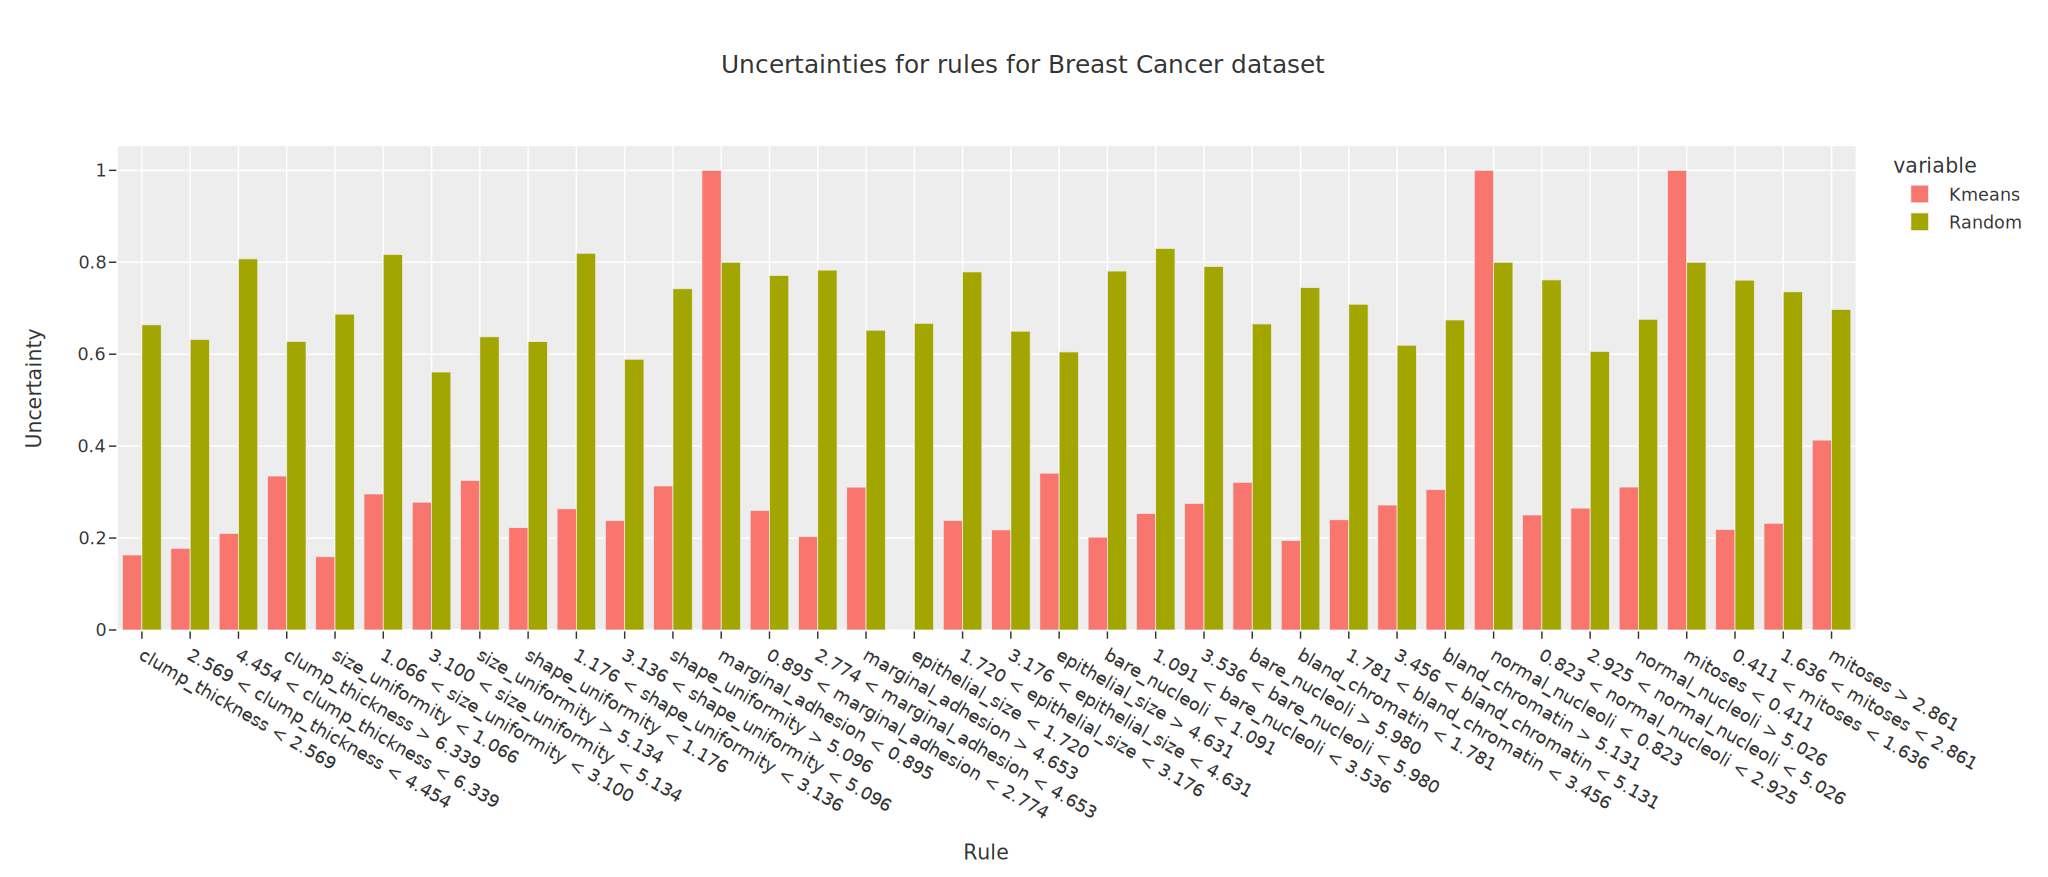
\includegraphics[width=\linewidth]{../../fig/bars.png}} 
    \caption{Uncertainties per rule for different MAF initialization methods}
    \label{fig:bars_uncertainty}
\end{figure}
\end{frame}

\begin{frame}{Bibliography}
\begin{thebibliography}{8}
{\rm
\bibitem{dst}
Shafer, G.: A Mathematical Theory of Evidence. Princeton University Press, Princeton (1976)

\bibitem{sergio}
Peñafiel, S., Baloian, N., Sanson, H., \& Pino, J. A.: Applying Dempster–Shafer theory for developing a flexible, accurate and interpretable classifier. Expert Systems with Applications \textbf{148}, 113262 (2020)

\bibitem{kmeans}
MacQueen, J.: Some Methods for Classification and Analysis of Multivariate Observations. Proc. 5th Berkeley Symp. on Math. Statist. and Prob., Vol. 1 (1967), 281--297

\bibitem{DBSCAN}
Ester, M., Kriegel, H.-P., Sander, J., Xu, X.: A density-based algorithm for discovering clusters in large spatial databases with noise. Proc. 2nd Int. Conf. on Knowledge Discovery and Data Mining (KDD'96), AAAI Press (1996), 226--231

\bibitem{Nelson}
Baloian, N., Davtyan, E., Petrosyan, K., Poghosyan, A., Harutyunyan, A., Penafiel, S.: Embedded Interpretable Regression using Dempster-Shafer Theory. Proceedings of the 4th Codassca Workshop on Data Science and Reliable Machine Learning (2024)

\bibitem{Aneta}
Baloyan, A., Aramyan, A., Baloian, N., Poghosyan, A., Harutyunyan, A., Penafiel, S.: An Empirical Analysis of Feature Engineering for Dempster-Shafer Classifier as a Rule Validator. Proceedings of the 4th Codassca Workshop on Data Science and Reliable Machine Learning (2024)
}
\end{thebibliography}
\end{frame}

\begin{frame}{Bibliography (continued)}
\begin{thebibliography}{8}
{\rm
\setcounter{enumiv}{6}
\bibitem{dsClustering}
Valdivia, R., Baloian, N., Chahverdian, M., Adamyan, A., Harutyunyan, A.: An Explainable Clustering Algorithm using Dempster-Shafer Theory. Proceedings of the 4th Codassca Workshop on Data Science and Reliable Machine Learning (2024)

\bibitem{breastCancer}
Wolberg, W. H., Mangasarian, O. L.: Multisurface method of pattern separation for medical diagnosis applied to breast cytology. Proceedings of the National Academy of Sciences \textbf{87}(23), 9193--9196 (1990)

\bibitem{brainTumor}
Bohaju, J.: Brain Tumor. In: Kaggle 2020, DOI: \doi{10.34740/KAGGLE/DSV/1370629}. \url{https://www.kaggle.com/dsv/1370629} (2020)

\bibitem{ripper}
Cohen, W.W.: Fast Effective Rule Induction. In: Prieditis, A., Russell, S. (eds.) Machine Learning Proceedings 1995, Morgan Kaufmann (1995), 115--123

\bibitem{czechs}
Sedláček, O., Bartoš, V.: Fusing Heterogeneous Data for Network Asset Classification – A Two-layer Approach. In: 2024 IEEE Network Operations and Management Symposium (NOMS) (2024)
}
\end{thebibliography}
\end{frame}

\begin{frame}{Paper and Code Availability}
\begin{center}
\begin{block}{Published Paper}
\textbf{DSGD++: Reducing Uncertainty and Training Time in the DSGD Classifier through a Mass Assignment Function Initialization Technique}
\\[0.5em]
\textit{Journal of Universal Computer Science}
\\[0.3em]
DOI: \doi{10.3897/jucs.164745}
\end{block}

\begin{block}{Source Code}
\textbf{Open Source Implementation}
\\[0.5em]
GitHub Repository: \\
\url{https://github.com/HaykTarkhanyan/DSGD-Enhanced}
\\[0.3em]
\textit{Complete implementation with datasets and experiments}
\end{block}
\end{center}
\end{frame}

\begin{frame}
    \begin{center}
        \Huge Thank you
    \end{center}
\end{frame}

\end{document}